\documentclass{neu_handout}
\usepackage{url}
\usepackage{amssymb}
\usepackage{amsmath}
\usepackage{marvosym}
\usepackage{graphicx}
\usepackage[pdftex]{graphicx}
\usepackage{subfigure}
\graphicspath{ {images/} }
\everymath{\displaystyle}

% Professor/Course information
\title{A Bayseian Approach to Fake News}
\author{Emily Dutile, Shubhi Mittal, Linghan Xing}
\date{December 2017}
\course{CS5100}{Foundations of AI}

\begin{document}
\section*{1 Introduction and Background}

"Fake news" became an increasingly coined term and was almost non-existent in the general context and media providers prior to October 2016 of the Presidential Election. In late 2016, the top 20 fake news stories on Facebook were reported to outperform the top 20 real news stories, which was determined by the number of comments, reactions, and shares. As seen in figure a, it is shown that the number of real news stories did not outperform the number of fake news stories towards the end of 2016. Undoubtedly, these stories and articles our shaping and influencing the thoughts and opinions of millions of individuals and companies need to step in to help stop the spread of fake news.
\\\\
With companies such as Facebook and Google who provide ad revenue to sites that host news stories, it should be the responsibility of these tech companies to be accountable for what content is displayed. Filtering out false information in order to correctly inform and educate our society, especially when it comes to presidential elections, is an extremely important and challenging task. Companies such as Signal Media have built AI-powered media monitoring in order to help this problem after they had discovered 'fake news' as being a headline in 27,000 articles over the course of the year (see figure b).

\begin{figure}[h]
\centering
\subfigure[BuzzFeed News]
{
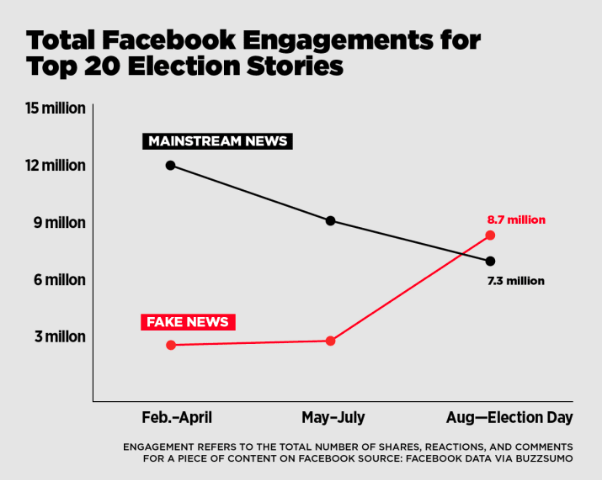
\includegraphics[width=0.3\linewidth]{buzzfeed}
}
\subfigure[]
{
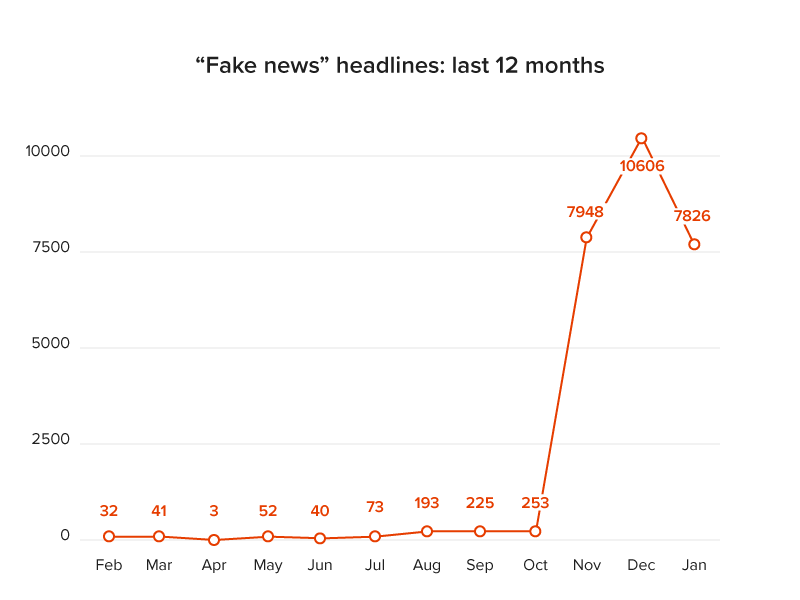
\includegraphics[width=0.3\linewidth]{fakenews}
}
\end{figure}

Fake news posts have exploited the feeds of Facebook users' which could deeply impact the options of our society if we loose our ability over time to decipher fake news from real news. Due to this problem, the data science community has looked to respond to this problem through a Kaggle competition called the Fake News Challenge \footnote{\url{http://www.fakenewschallenge.org}}. Determining real news from fake news is an extremely challenging task within the machine learning and natural language processing community. Creating models that accurately filter out fake news without removing real news sources is a very complicated task due to how we define fake news itself in order to correctly label real and fake news.\\

In our approach to tackle this problem, we wanted to combat fake news by implementing a bayesian model that can differentiate fake news from real news. Expanding on this original approach, we have implemented several supervised machine learning based algorithms using the scikit-learn package in order to compare text classifiers on fake news recognition. 


\subsection*{1.1 The Data}
As mentioned previously, what makes this challenge interesting and hard is around the very definition of fake news. Since we did not want to be caught up in the process of deciphering, scraping the web, and labeling fake news vs. real news, we found a dataset that contains over 6,000 articles that are tagged as either real or fake news \footnote{\url{https://github.com/GeorgeMcIntire/fake_real_news_dataset}}. The fake news in this dataset is from the Kaggle fake news data set\footnote{\url{https://www.kaggle.com/mrisdal/fake-news}} that was released from the 2016 election.

The real news was aquired through web scraping articles off of All Sides, which is a website that is dedicated to hosting news from across the political spectrum. The articles that were chosen for the real dataset came from media organizations such as the New York Times, WSJ, Bloomberg, NPR, and the Guardian. These were all published in 2015 and 2016. The dataset is constructed with almost equal parts which gives the models null accuracy to be about 50 percent. The number of articles that are identified as real is 3171, and the number of articles identified as fake is 3164. The data set seems to follow the definition of fake news provided by First Draft News comprises of 7 types of fake content: false connection, false context, manipulated content, satire or parody, misleading content, imposter content, and fabricated content. We started by separating the labels and set up training data and testing data.


\subsection*{1.2 Methods}
We performed supervised machine learning techniques such as multinomial bayes, SVM, random forest and logistic regression. Out of these models, we implemented our own multinomial naive bayes algorithm and abstracted linguistic features using NLTK. For feature extraction, we implemented our own bag-of-words (count vectorizor) and Term Frequency–Inverse Document Frequency (TF-IDF), but also used the scikit-learn versions when using the out-of-the-box models. SVM, Random Forest, and linear regression were all run in order to compare the accuracy and output to our model. With respect to language processing, tokenization, filtering, lemmatization, and stemming were all used for preprocessing the titles and body text of the articles in the data set. For our evaluation process, we used a confusion matrix to understand the accuracy of our models.

\subsection*{1.3 Related Work}
Within the industry, companies such as Facebook have stumbled in this combat, mostly relying on users reporting fake news and outsourcing this task to third parties in order to remove direct bias. Identifying and labeling the data itself is the extreme complexity around this issue in industry. With respect to our implementation, receiving a data set that has already been labeled with fake news and real news does take that complexity out of the issue at hand. This process in itself is very complex and may take multiple steps. Interestingly enough, Facebook has found that users who post a signification amount, about 50 times or more a day, are most likely shares news or posts that the company has identified as fake. With this approach taken in to consideration, it may be a possible piece of the solution in order to lessen the distribution of fake news. In another test, Facebook created a test that prioritized comments to the top of news feed that had the word 'fake' in it. Although the company as made a few attempts and run some tests so far, it's clear that this is no easy task and can certainly annoy users.

\begin{figure}[h]
\centering
{
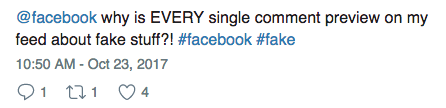
\includegraphics[width=0.3\linewidth]{fbfake}
}
\end{figure}

With in the Fake News Challenge, teams were tasked with assessing the veracity of a news story by identifying fake news through Stance Detection as a building block for fact-checking. The challenge defines stance detection as "estimating the relative perspective (or stance) of two pieces of text relative to a topic, claim or issue". With in this data set, the input was a headline and body of text, and the output would classify the stance of the body text relative to the claim in the headline. The four categories were:\\
Agrees: The body text agrees with the headline.\\
Disagrees: The body text disagrees with the headline.\\
Discusses: The body text discuss the same topic as the headline, but does not take a position\\
Unrelated: The body text discusses a different topic than the headline\\

With respect to labeling the stance of an article to then determine if it is real or fake is a difficult task of this entire process. Some of the top teams that participated in the Fake News Challenge ended up using neural networks to get the best results. The number one team, SOLAT in the SWEN\footnote{\url{https://github.com/Cisco-Talos/fnc-1}}, received the best results using a weighted average between gradient-boosted decision trees and a deep convolutional neural network. The combination of these two approaches detected the correct stance for each headline, which gave the team a relative score of 82.02 in the competition. Looking at the models that many teams had to use in order to receive the best results, we were not expecting our naive bayes model to produce the best results. However, we felt that on this dataset it was a good implementation when coupled with proper language processing and feature extraction techniques since our articles were already labeled as either real or fake.

\section*{2 Supervised Approach}

\subsection*{2.1 Feature Extraction}

For feature extraction, we used the body text of the articles in the data set and ignored the titles. We thought that using the longer text would allow for distinct words and features from the data set. For understanding if the words and tokens in the articles text had a significant impact on whether the news was fake or real.\\

Given a list of documentations, feature extraction converts each of the documents into a list of features, generating a sparse matrix for our Naive Bayes model. Features from our text classifier could include anything from manually created labels to the occurrence of words in the texts. In our case the naive assumption is that given that fact that a document is fake or authentic, the occurrence of each word is independent from each other. To implement our feature extraction, we first extracted words from the documents/text. To do this, we used stop words, tokenization, and stemming.\\

English stop words were removed from the data for better results. Stop words are frequent in our natural language but usually doesn't have additional information, such as words like "a", "on", "this", "the", "is", etc. By removing them the distraction in the vocabulary is usually reduced. In tokenization, the document is tokenized into a list of words, with all the punctuation being taken away and making all words lower case. In stemming, the words that have the same roots are assigned to the same root word. For example: "attack", "attacking" and "attacked" will be categorized as the same root word, "attack".

\subsubsection*{2.1.1 Count Vectorization}

After the word list for each document is built, a vocabulary can be established by looping through the documents and finding the set of words that occurred. This is often referred as "bag-of-words". Until this point, we have 'sanitized' our input text and can start building the count vector. There are two approaches that we implemented to get the term frequency matrix: naive boolean term frequency and logarithmic term frequency. The naive boolean term frequency is the simple way of counting the occurrence of each word in the vocabulary and simply assigning their occurrences in the matrix. This method is easier to implement and in many case yields reasonable results. In the second approach, we assume that the correlation between how important a word is a how many times the word occurs in the text should not be linear. If the word "love" occurred 4 times in a text, this does not mean that the author "loves" 4 times more than one who only used "love" once in their text. Therefore a possible improvement to that is to use logarithmic occurrence:
$$Frequency(w,d) = 1 + log(word_count)$$
 
To compare the results of our implementation, CountVectorizer was also used from the scikit-learn package and in this stage no weighting is assigned to any of these words.


\subsubsection*{2.1.2 TF-IDF}
In addition to the counting of term frequency, some words will occur very frequently in the documents to a point that the occurrence of them does not provide much additional information. For example, if the word "American" is present in every text, then the occurrence of this word does not provide any information for our classifier. In such circumstances the inverse document-frequency (IDF) is a common practice method to weight on the term frequency.

$$idf(w,D)=log((1+n_d)/(1+df(d,t)))+1$$

In the resulting matrix, we apply the idf with the generated tf to produce a weighted vector, this is called TF-IDF:

$$tf-idf(w)=tf(w)*idf(w)$$

Note that the 1 is there as a 'smoothing factor' to address the situation that the denominator is 0. The final step of our feature extraction is to normalize the TF-IDF matrix so that the resulting variance between each word are reduced to reflect their weighted value.\\

TfidfVectorizor from the scikit-learn package was used with a max threshold set at 0.7 in order to remove words which appear in more than 70 percent of the articles. Before buildings the vectors, we removed English stop words from the data set and performed tokenization and stemming.

\subsection*{2.2 Models}



\subsubsection*{2.2.1 Multinominal Naive Bayes}

A multinomial Naive Bayes model is a classic solution to the text classification problem described here due to the reasons that: the classes here are discrete, i.e. Fake or Real; the occurrence of words is largely considered independent given the class of a document (although certain patterns of the words, such as ‘Donald Trump’, ‘U.S. Congress’, could be further extracted as features); and it in a lot cases yields reasonable accuracy.\\

For our implementation of a Multinomial Bayes classifier, we segregated the data corpus with 70 percent of it used for the purpose of training and 30 percent of it used for the purpose of accuracy estimation. We first tokenize the text by using  natural language processing techniques which includes word stemming and stop words removal. This is done for all news sample in the entire training corpus to generate a vocabulary of unique words. The entire vocabulary of unique words constitutes as features. In our implementation of Naive Bayes, we find the frequency distribution of each word in the vocabulary for the given class i.e. fake/real. The trained model is a word-label count matrix of size $|V|*|L|$ where $|V|$ is the size of the vocabulary and $|L|$ is the number of labels. \\\\

Below is a sample of the trained model:

\begin{table}[h]
\centering
\begin{tabular}{l*{6}{c}r}
Vocabulary     & FAKE & REAL \\
\hline
trump 			& 128 & 1024   \\
truce            & 256 & 32  \\
israel           & 512 & 2048  \\
president     & 16 & 64  \\
\end{tabular}\\
\end{table}

For testing, each news sample is transformed to the tokens as explained above and for each word token the probability of the word given a label class is calculated using the following formulae:

$$P(w|c) = (count(w, c) + f(s))/(count(c) + |V|)$$

Where c is the class which can be either fake or real. P(w|c) is the probability of the word given class c. count(w, c) is the count of word w in the class c which is obtained by look up in the trained model. count(c) is the count of all the words in the class c. |V| is the size of vocabulary. f(s) is the smoothening factor  which is 1 in our case. smoothening is done to reduce the impact of unseen words in the trained corpus.\\

The final probability of classification is formulated by taking the product of all of the P(w|c) for each token:\\
$$P(sample|fake) = P(fake) * P(w|fake)$$ for all w belonging to the sample
$$P(sample|real) = P(real) * P(w|real)$$ for all w belonging to the sample
$$P(sample|c) = max(P(sample|fake), P(sample|real))$$


\subsubsection*{2.2.2 Support Vector Machines}

Although not as computationally fast as naive bayes, a linear support vector machine is widely known as one of the best  algorithms for text classification. It's a great binary classifier since it generates a hyperplane which separates the training data as far as possible, so it performs well with a high number of features. In further explorations of this project we would like to implement it ourselves, but due to time constraints we used the scikit-learn SVM model using our features extracted with TF-IDF and trained it with the data. As expected, we received the best results using this model with a 93 percent accuracy. Using the bag-of-words approach for feature extraction resulted in an 87 percent accuracy.



\subsubsection*{2.2.3 Random Forest}

A random forest builds a number of decision trees at training time and then outputs the class that is the mode of the classes or the mean prediction of the individual trees. In a decision tree, we have a set of nodes with the structure of a tree graph. Starting at the root, a decision is made, and then at each node the input input is tested. From the outcome that we get from this, we then go on to the next node. If a node is a leaf then that is the decision, being either real news or fake news. A random forest was tried as a classifier for the same training data set and test data set. It
yielded a lower accuracy value than all of the models except multinomial naive bayes TF-IDF. Our model using a Random Forest Classifier achieves an accuracy of roughly 83 percent when using features such as TF-IDF and count vector. Although features can be dependent for this model, since there are a large number of spare features, we believed that this caused overfitting and resulted in a lower accuracy.
 
 
\subsubsection*{2.2.4 Logistic Regression}
Unlike SVMS, Logistic regression allows probabilities to be modeled, and unlike naive bays, features can be dependent, so we originally believed that this would give fairly accurate results. It takes a probabilistic approach to learning discriminative functions. Each word feature $x_i$ is given a weight $w_i$. With the following logistic function, we can represent the probability for each fake or real classification:

$$P(c = real | x_1, x_2,..x_n) = \frac{1}{1 + e^{w_0 + \sum^n w_i x_i}} $$

$$P(c = fake | x_1, x_2,..x_n) = 1 - P(c = real | x_1, x_2,..x_n) = \frac{e^{w_0 + \sum^n w_i x_i}}{1+e^{w_0 + \sum^n w_i x_i}}$$

where $w_0$ is the bias.

\section*{3 Evaluation}

In order to evaluate our models, we calculated the accuracy. The accuracy of the naive bayes model that we implemented was almost percent, which was what we were expecting on this data set. In comparison to the sklearn MNB implementation, we were only off by 1 percent accuracy. We believe this could be because of how we did our preprocessing and feature extraction, and further adjustments could have resulted in a more accurate model. If we used the same model on the Fake News Stance challenge, we believe that this would result in a far lower accuracy considering the complexity of the models that the teams had used. Properly trained Naive Bayes classifiers are usually astonishingly accurate and fairly quick to train, so we were expected decent results, but not the best. The accuracy results of all of our results can be see below:

\begin{table}[h]
\centering
\begin{tabular}{l*{6}{c}r}
Model     & Accuracy  \\
\hline
Naïve Bayes  (own implementation) & .878   \\
Multinomial Naïve Bayes (CV)       & .888  \\
Multinomial Naïve Bayes (TF-IDF)      & .835  \\
Random Forest (CV)     & .839  \\
Random Forest (TF-IDF)     & .838  \\
SVM (CV)     & .87  \\
SVM (TD-IDF)     & .93  \\
Linear Regression (CV)  & .851 \\
Linear Regression (TF-IDF)  & .923 \\
\end{tabular}\\
\end{table}



To evaluate the different models and our results, we created a confusion matrix for each model in order to describe the performance of the classifier on the test data since we know the 'true'/original label.\\

We originally anticipated that feature extraction using TF-IDF would give better results for all models. However, using the bag-of-words approach with the MNB model proved to be a fast and fairly accurate approach in the indentification of fake and real news with this dataset. MNB using TF-IDF proved to be the classifier that was least correct. Interestingly enough, it seemed that stemming an lemmatization slightly decreases the accuracy of prediction for all models. The fake news detection system that achieved the highest accuracy and best evaluation was the SVM using TF-IDF, and logistic regression with almost the same accuracy.

\begin{figure}[h]
\centering
\subfigure[MNB (Count Vector)]
{
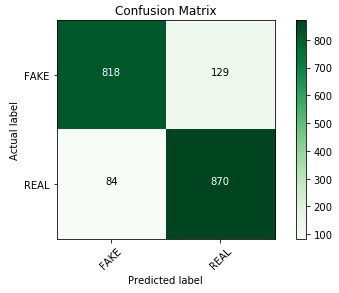
\includegraphics[width=0.2\linewidth]{nb_cv}
}
\subfigure[MNB (TF-IDF)]
{
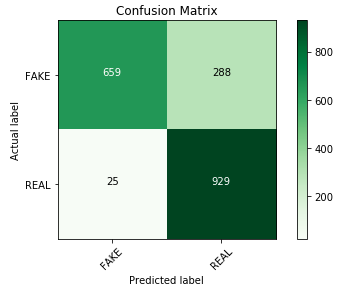
\includegraphics[width=0.2\linewidth]{nb_tfidf}
}
\subfigure[Random Forest (CV)]
{
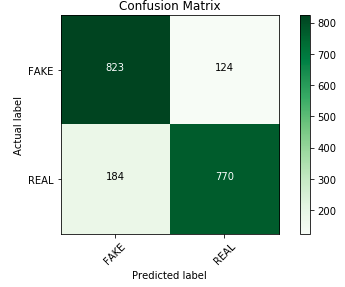
\includegraphics[width=0.2\linewidth]{rf_cv}
}
\subfigure[Random Forest (TF-IDF)]
{
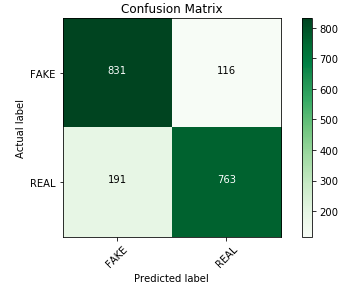
\includegraphics[width=0.2\linewidth]{rf_tfidf}
}
\end{figure}

\begin{figure}[h]
\centering
\subfigure[SVM (Count Vector)]
{
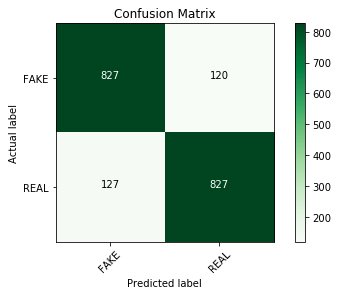
\includegraphics[width=0.2\linewidth]{svm_cv}
}
\subfigure[SVM (TF-IDF)]
{
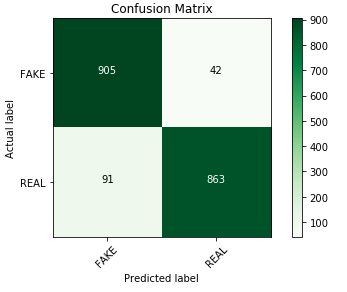
\includegraphics[width=0.2\linewidth]{svm_tfidf}
}
\subfigure[Linear Regression (CV)]
{
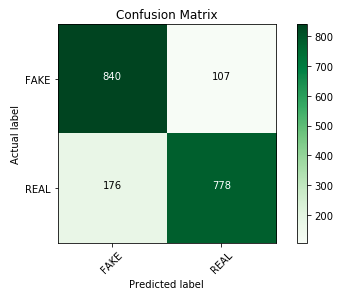
\includegraphics[width=0.2\linewidth]{reg_cv}
}
\subfigure[L. Regression (TF-IDF)]
{
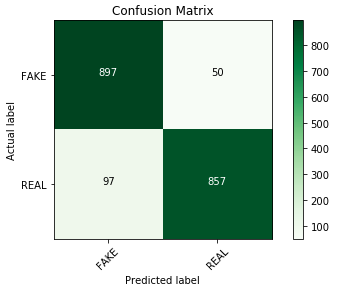
\includegraphics[width=0.2\linewidth]{reg_tfidf}
}
\end{figure}


\section*{4 Acknowledgments}

The entire team participated in the implementation of the naive bayes model, presentation and writing the report. With respect to feature extraction, Linghan did the majority of the work. Shubhi took on the preprocessing, including stemming and tokenization with the use of NLTK. Emily prepared the evaluations and also wrote the code to train the other models for comparisons. Finally, we would like to thank Prof. Stacy and Dan Feng for their direction and guidance during this project.

\section*{5 Discussion}
As we have observed, the classification results produced by our naive bayes implementation are fairly satisfying. Although naive bayes is one of the easier machine learning algorithms to implement, we encountered the problems and difficulties with a lot of natural language processing and how feature extraction is extremely important in order to get the best results from the model. When running our models with shorter text articles, such as the titles/headings of the documents, we found that the results were less accurate overall. It would be interesting to further explore how our model runs against other datasets and we would like to continue exploration around stance detection in fake news.\\

Through our implementations and attempts to combat fake news, it is clear that this is no easy task, but it looks to be a solvable problem using artificial intelligence, machine learning, and natural language processing if we can find the building blocks to accurately identify and label fake news. With the increasing amount of articles on the internet, preprocessing the data and extracting features is extremely important and difficult.


\begin{thebibliography}{9}

\bibitem{ai} 
Russel and Norvig. 
\textit{Artificial Intelligence: A Modern Approach, 3rd Ed.}. 

 
\bibitem{buzzfeed}  
\textit{This Analysis Shows How Viral Fake Election News Stories Outperformed Real News on Facebook}.
[\textit{BuzzFeed News, November 2016}].
\url{https://www.buzzfeed.com/craigsilverman/viral-fake-election-news-outperformed-real-news-on-facebook?utm_term=.tnpJN34BM#.yfV6V10ZX}.
 

\bibitem{Signal}  
\textit{12 Months of Fake News Headlines, Dissected with Media Monitoring}. 
 \url{https://signalmedia.co/media-monitoring-blog/fake-news-dissected-media-monitoring/}.

\bibitem{firstdraftnews}  
\textit{Facebook's fake news experiment backfires}.
[\textit{BBC News}]. 
 \url{https://firstdraftnews.com/fake-news-complicated}.
 
 
\bibitem{bbc}  
\textit{Fake News. It's Complicated}.
[\textit{BBC News}]. 
 \url{http://www.bbc.com/news/technology-41900877}.
 
\bibitem{talos}  
\textit{Talos Targets Disinformation with Fake News Challenge Victory}.
[\textit{Talos Intelligence}]. 
 \url{https://blog.talosintelligence.com/2017/06/talos-fake-news-challenge.html}.
 
\bibitem{nb}  
\textit{The Optimality of Naive Bayes}.
[\textit{Harry Zhang}]. 
 \url{http://www.cs.unb.ca/~hzhang/publications/FLAIRS04ZhangH.pdf}.
 
 
\bibitem{rf}  
\textit{Multinomial Naive Bayes}.
[\textit{
Rafael Merino García}]. 
 \url{https://www.youtube.com/watch?v=km2LoOpdB3A&t=424s}.
 
\bibitem{fb}
\textit{Facebook found a new way to identify spam and false news articles in your News Feed}
[\textit{
Kurt Wagner}]. 
 \url{https://www.recode.net/2017/6/30/15896544/facebook-fake-news-feed-algorithm-update-spam}.

\bibitem{ml} 
Kevin Murphy. 
\textit{Machine Learning, A Probabilistic Perspective.}.

\bibitem{ml2} 
Ethem Alpaydin. 
\textit{Introduction in Machine Learning}.

\end{thebibliography}


\end{document}